
\documentclass[10pt,journal,compsoc]{IEEEtran}


% *** CITATION PACKAGES ***
%
\ifCLASSOPTIONcompsoc
  % IEEE Computer Society needs nocompress option
  % requires cite.sty v4.0 or later (November 2003)
  \usepackage[nocompress]{cite}
\else
  % normal IEEE
  \usepackage{cite}
\fi

%\usepackage{tensor}
\usepackage{psfrag}
\usepackage{amsmath,amsfonts,amssymb}
\usepackage{array,delarray}
\usepackage[dvips]{graphicx, color}
%\usepackage{dsfont}
%\usepackage[square,sort&compress]{natbib}
%\usepackage{indentfirst}
\usepackage{algorithm}
\usepackage{enumerate}
\usepackage[noend]{algorithmic}
\usepackage{url}
%\algsetup{indent=1.5em}
\newcommand{\given}{\mbox{ | }}
%
\newtheorem{theorem}{Theorem}[section]
\newtheorem{corollary}[theorem]{Corollary}
\newtheorem{lemma}[theorem]{Lemma}

\newenvironment{proof}[1][Proof]{\begin{trivlist}
\item[\hskip \labelsep {\bfseries #1}]}{\end{trivlist}}
\newenvironment{definition}[1][Definition]{\begin{trivlist}
\item[\hskip \labelsep {\bfseries #1}]}{\end{trivlist}}
\newenvironment{example}[1][Example]{\begin{trivlist}
\item[\hskip \labelsep {\bfseries #1}]}{\end{trivlist}}
\newenvironment{remark}[1][Remark]{\begin{trivlist}
\item[\hskip \labelsep {\bfseries #1}]}{\end{trivlist}}

\newcommand{\red}[1]{\textcolor{red}{#1}}
% correct bad hyphenation here
\hyphenation{op-tical net-works semi-conduc-tor}
\newcommand{\algo}{\textsc{SAHad}}


\begin{document}

\title{MapReduce Based Subgraph Counting: variations and performance study}

\author{{Zhao~Zhao, Meng~Li, Guanying~Wang, Ali~Butt, Maleq~Khan, \\
	Madhav~Marathe, Judy~Qiu, Anil~Vullikanti}% <-this % stops a space

\IEEEcompsocitemizethanks{

	\IEEEcompsocthanksitem Zhao Zhao, Madhav Marathe and Anil Vullikanti are
	with the Biocomplexity Institute of Virginia Tech
and the Department of Computer Science, Virginia Tech, VA, 24061.\protect\\
% note need leading \protect in front of \\ to get a newline within \thanks as
% \\ is fragile and will error, could use \hfil\break instead.
	E-mail: zhaozhao@vt.edu, mmarathe@vt.edu, vsakumar@vt.edu 

	\IEEEcompsocthanksitem Ali~Butt is
	with the Department of Computer Science, Virginia Tech, VA, 24061.\protect\\
% note need leading \protect in front of \\ to get a newline within \thanks as
% \\ is fragile and will error, could use \hfil\break instead.
	E-mail: butta@cs.vt.edu

	\IEEEcompsocthanksitem Maleq Khan is with the Department of Electrical Engineering and Computer Science,
	Texas A\&M University-Kingsville. \protect\\ 
	E-mail: maleq.khan@tamuk.edu

	\IEEEcompsocthanksitem Meng Li and Judy Qiu are with the Intelligent Systems
	Engineering, Indianna University. \protect\\
	Email: li526@umail.iu.edu, xqiu@indiana.edu

	\IEEEcompsocthanksitem Guanying Wang is working with Google Inc. \protect\\
	Email:wang.guanying@gmail.com}% <-this % stops an unwanted space

}

% note the % following the last \IEEEmembership and also \thanks - 
% these prevent an unwanted space from occurring between the last author name
% and the end of the author line. i.e., if you had this:
% 
% \author{....lastname \thanks{...} \thanks{...} }
%                     ^------------^------------^----Do not want these spaces!
%
% a space would be appended to the last name and could cause every name on that
% line to be shifted left slightly. This is one of those "LaTeX things". For
% instance, "\textbf{A} \textbf{B}" will typeset as "A B" not "AB". To get
% "AB" then you have to do: "\textbf{A}\textbf{B}"
% \thanks is no different in this regard, so shield the last } of each \thanks
% that ends a line with a % and do not let a space in before the next \thanks.
% Spaces after \IEEEmembership other than the last one are OK (and needed) as
% you are supposed to have spaces between the names. For what it is worth,
% this is a minor point as most people would not even notice if the said evil
% space somehow managed to creep in.



% The paper headers
\markboth{IEEE Transactions on Multi-Scale Computing Systems}%
{Shell \MakeLowercase{\textit{et al.}}:MapReduce Based Subgraph Counting:
Variations and Performance Study}

% The only time the second header will appear is for the odd numbered pages
% after the title page when using the twoside option.
% 
% *** Note that you probably will NOT want to include the author's ***
% *** name in the headers of peer review papers.                   ***
% You can use \ifCLASSOPTIONpeerreview for conditional compilation here if
% you desire.



% The publisher's ID mark at the bottom of the page is less important with
% Computer Society journal papers as those publications place the marks
% outside of the main text columns and, therefore, unlike regular IEEE
% journals, the available text space is not reduced by their presence.
% If you want to put a publisher's ID mark on the page you can do it like
% this:
%\IEEEpubid{0000--0000/00\$00.00~\copyright~2015 IEEE}
% or like this to get the Computer Society new two part style.
%\IEEEpubid{\makebox[\columnwidth]{\hfill 0000--0000/00/\$00.00~\copyright~2015 IEEE}%
%\hspace{\columnsep}\makebox[\columnwidth]{Published by the IEEE Computer Society\hfill}}
% Remember, if you use this you must call \IEEEpubidadjcol in the second
% column for its text to clear the IEEEpubid mark (Computer Society jorunal
% papers don't need this extra clearance.)



% use for special paper notices
%\IEEEspecialpapernotice{(Invited Paper)}



% for Computer Society papers, we must declare the abstract and index terms
% PRIOR to the title within the \IEEEtitleabstractindextext IEEEtran
% command as these need to go into the title area created by \maketitle.
% As a general rule, do not put math, special symbols or citations
% in the abstract or keywords.
\IEEEtitleabstractindextext{%

\begin{abstract}

Subgraph isomorphism and its variants are commonly arising problems in a number of
real world applications, such as genetic network analysis in
bioinformatics, web analysis, disease diffusion prediction and social network
analysis. These problems are computationally very challenging to scale to
very large networks with millions of nodes. In this paper, we present \algo{}, a novel
MapReduce based algorithm for detecting and counting trees of bounded size using the color coding
technique, developed by N. Alon, R. Yuster and U. Zwick, Journal of the ACM (JACM) 1995.
\algo{} is a randomized algorithm and we show
rigorous bounds on the approximation quality and the performance. We implement
\algo{} on two different frameworks: the standard Hadoop model and Harp, a more power
computing environment, and evaluate its performance on a variety of synthetic and
real networks. \algo{} scales to very large networks with
up to tens of millions of nodes and 0.5 billion edges and trees of up to 12 nodes.
Further, our Harp based implementation gives an order of magnitude improvement
in performance over the standard Hadoop implementation.


%Subgraph analysis and subgraph isomorphism detection are key components in many
%real world applications that are underlyingly modeled by graph operations. Such
%applications include but not limited to: genetic network analysis in
%bioinformatics, web analysis, disease diffusion prediction, social network
%modeling, etc. However, it is computationally very challenging to perform
%subgraph analysis and isomorphism detection in those applications, due to the
%massive size of the network, which normally ranges from millions to billions of
%nodes, and the nature of the problem, which is NP-hard. In this paper, we
%explore how to efficiently perform the computation in a parallel environment, by
%deducing the subgraph counting problem into a MapReduce problem. Theoretical
%analysis shows that the worst case work complexity is asymptotically very close
%to that of the best sequential algorithm. We also perform rigorous experimental
%study on various graphs with different frameworks including Hadoop and Harp. The
%experimental results show that our algorithm scales to very large networks with
%up to tens of millions of nodes and 0.5 billion edges. In addition, the Harp
%based implementation achieves a performance improvement by an order of magnitude
%over the Hadoop based.

\end{abstract}

% Note that keywords are not normally used for peerreview papers.
\begin{IEEEkeywords}
subgraph isomorphism, graph partitioning, MapReduce, Hadoop, Harp
\end{IEEEkeywords}}


% make the title area
\maketitle


% To allow for easy dual compilation without having to reenter the
% abstract/keywords data, the \IEEEtitleabstractindextext text will
% not be used in maketitle, but will appear (i.e., to be "transported")
% here as \IEEEdisplaynontitleabstractindextext when the compsoc 
% or transmag modes are not selected <OR> if conference mode is selected 
% - because all conference papers position the abstract like regular
% papers do.
\IEEEdisplaynontitleabstractindextext
% \IEEEdisplaynontitleabstractindextext has no effect when using
% compsoc or transmag under a non-conference mode.



% For peer review papers, you can put extra information on the cover
% page as needed:
% \ifCLASSOPTIONpeerreview
% \begin{center} \bfseries EDICS Category: 3-BBND \end{center}
% \fi
%
% For peerreview papers, this IEEEtran command inserts a page break and
% creates the second title. It will be ignored for other modes.
\IEEEpeerreviewmaketitle


\IEEEraisesectionheading{\section{Introduction}\label{sec:introduction}}
% Computer Society journal (but not conference!) papers do something unusual
% with the very first section heading (almost always called "Introduction").
% They place it ABOVE the main text! IEEEtran.cls does not automatically do
% this for you, but you can achieve this effect with the provided
% \IEEEraisesectionheading{} command. Note the need to keep any \label that
% is to refer to the section immediately after \section in the above as
% \IEEEraisesectionheading puts \section within a raised box.




% The very first letter is a 2 line initial drop letter followed
% by the rest of the first word in caps (small caps for compsoc).
% 
% form to use if the first word consists of a single letter:
% \IEEEPARstart{A}{demo} file is ....
% 
% form to use if you need the single drop letter followed by
% normal text (unknown if ever used by the IEEE):
% \IEEEPARstart{A}{}demo file is ....
% 
% Some journals put the first two words in caps:
% \IEEEPARstart{T}{his demo} file is ....
% 
% Here we have the typical use of a "T" for an initial drop letter
% and "HIS" in caps to complete the first word.
% You must have at least 2 lines in the paragraph with the drop letter
% (should never be an issue)

\IEEEPARstart{G}{iven} two graphs $G$ and $H$, the subgraph isomorphism problem
asks if $H$ is isomorphic to a subgraph of $G$. The counting problem associated
with this seeks to count the number of copies of $H$ in $G$. These and other
variants are fundamental problems in Network Science and have a wide range of
applications in areas such as bioinformatics, social networks, semantic web,
transportation and public health.  Analysts in these areas search for meaningful
patterns in networked data; often, these patterns are specific subgraphs such as
trees.  Three different variants of subgraph analysis problems have been studied
extensively.  The first version involves counting specific subgraphs, which has
applications in bioinformatics~\cite{alon2008biomolecular,
huffner2008algorithm}.  The second involves finding the most frequent subgraphs
either in a single network or in a family of networks---this has been used in
finding patterns in bioinformatics (e.g.,~\cite{kuramochi2005finding}),
recommendation networks~\cite{leskovec2006patterns}, chemical structure
analysis~\cite{raymond2002maximum}, and detecting memory
leaks~\cite{maxwell2010diagnosing}. The third involves finding subgraphs which
are either over-represented or under-represented, compared to random networks
with similar properties---such subgraphs are referred to as ``motifs''. Milo et
al. ~\cite{milo2002network} identify motifs in many networks, such as
protein-protein interaction (PPI) networks, ecosystem food webs and neuronal
connectivity networks. Subgraph counts have also been used in characterizing
networks~\cite{przulj2007biological}.

Subgraph Isomorphism problem and its variants are well known to be
computationally challenging.  In general the decision version of the problem is
{\sf NP}-hard, and the counting problem is \#{\sf P}-hard.  Extensive work has
been done in theoretical computer science on this problem; we refer the reader
to the recent papers
by~\cite{marx2014everything,flum2004parameterized,curticapean2014complexity} for
an extensive discussion on the decision and counting complexity of the problem
and tractable results for various parameterized versions of the problem.

The primary focus of this paper is on the three mentioned variants of the
subgraph isomorphism problem when $k$, the number of nodes in the template $H$,
is fixed. Letting $n$ be the number of nodes in $G$, one can immediately get
simple algorithms with running time $O(n^k)$ to find and count the number of
copies of template $H$ in $G$. Note that in this paper we focus on non-induced
subgraph matching.
%These are computationally very challenging problems, and there has been a lot
%of work on finding a subgraph (also referred to as a ``template'') of size $k$
%in a graph with $n$ nodes.  Eisenbrand \emph{et al}.
%~\cite{eisenbrand2004complexity} developed an algorithm with a running time of
%roughly $O(n^{\omega k/3})$ (which improves on the naive $O(n^k)$ time
%algorithm), where $\omega$ denotes the exponent of the best possible matrix
%multiplication algorithm. If the template has an independent set of size $s$,
%Vassilevska \emph{et al}.  \cite{vassilevska2009finding} give an algorithm with
%an improved running time of $O(2^sn^{k-s+3}k^{O(1)})$; this is improved
%slightly by Kowaluk \emph{et al}.  \cite{kowaluk2011counting}. 
When the template is a tree or has a bounded treewidth, Alon \emph{et
al}.~\cite{alon2008biomolecular} present an elegant randomized approximation
algorithm with running time
$O(k|E|2^ke^k\log{(1/\delta)}\frac{1}{\varepsilon^2})$, where $\varepsilon$ and
$\delta$ are error and confidence parameters, respectively, based on the color
coding technique.  There result was  significantly improved by Koutis and
Williams~\cite{koutis2009limits} who gave an algorithm with running time of
$O(2^k|E|)$.

A lot of practical heuristics have also been developed for various versions of
these problems, especially for the frequent subgraph mining problem. An example
is the ``Apriori'' method, which uses a level-wise exploration of the template
\cite{inokuchi2000apriori, kuramochi2005finding}, for generating candidates for
subgraphs at each level; these have been made to run faster by better pruning
and exploration techniques, e.g.,~\cite{kuramochi2005finding, huan2004spin,
yan2005mining}. Other approaches in relational databases and data mining involve
queries for specific labeled subgraphs, and have combined relational database
techniques with careful depth-first exploration, e.g.,~\cite{sakr2009graphrel,
ronen2009evaluating, brocheler2010cosi}.

Most of these approaches are
sequential, and generally  scale to modest size graphs $G$  and templates $H$.
Parallelism is necessary to scale to much larger networks and templates.
In general, these approaches are  hard to parallelize as it is 
difficult to decompose the task into independent subtasks. It is not clear if
candidate generation approaches~\cite{kuramochi2005finding, huan2004spin,
yan2005mining} can be parallelized and scaled to large graphs and computing
clusters. Two recent approaches for parallel algorithms, related to this work,
are~\cite{brocheler2010cosi, zhao2010subgraph}. The approach of Br\"{o}cheler
\emph{et al}. ~\cite{brocheler2010cosi} requires a complex preprocessing and
enumeration process, which has high end-to-end time, while the approach of
\cite{zhao2010subgraph} involves an MPI-based implementation with a very high
communication overhead for larger templates.  Two other papers
\cite{suri2011counting, pagh2011colorful} develop MapReduce based algorithms for
approximately counting the number of triangles with a work complexity bound
$O(|E|)$. The development of  parallel algorithms for
subgraph analysis with rigorous polynomial work complexity, which are
implementable on heterogeneous computing resources remains an open problem.
Due to the complexity of
enumerating subgraphs, people propose to compute some metrics of the subgraph
which is anti-monotune to the subgraph size. The algorithm  reported in
\cite{abdelhamid2016scalemine} is capable of computing subgraph support on
 large network with up to 1 Billion edges. However, it requires each
machine to have a copy of the graph in memory which limits its scalability to larger graphs.
Additionally, computing support requires much less computational effort
than counting subgraphs. Another recent work also employs MapReduce to match
subgraph~\cite{suo2016towards} which scales to networks with up to 300 million
edges. 

Other approaches studied in the context of data mining and databases,
e.g.,~\cite{sakr2009graphrel, ronen2009evaluating, brocheler2010cosi},
are capable of processing large networks, but are usually slow due to
limitations of database techniques for processing networks.

\noindent
\textbf{Our contributions}.
In this paper, we present \sahad{}, a new algorithm for
\underline{S}ubgraph \underline{A}nalysis using \underline{Had}oop, with
rigorously provable polynomial work complexity for several variants of the subgraph
isomorphism problem when $H$ is a tree.
\sahad{} scales to very large graphs, and because of the Hadoop
implementation, runs flexibly on a variety of computing resources, including
Amazon EC2 cloud. Our specific contributions are discussed below.


%\begin{enumerate}
%\item

\smallskip
\textbf{1.} \sahad{} is the first MapReduce-based algorithm for finding and
counting labeled trees in very large networks.
The only prior Hadoop based approaches have been on triangles
\cite{tsourakakis2009doulion, pagh2011colorful, suri2011counting} in very large
networks, or more general subgraphs on relatively small networks
\cite{liu2009mapreduce}. Our main technical contribution is the development of a
Hadoop version of the \emph{color coding}
algorithm of Alon \emph{et al}.~\cite{alon2008biomolecular, alon1995color}, which
is a (sequential) randomized approximation algorithm for subgraph counting.
It is a randomized approximation algorithm that for any $\varepsilon, \delta$,
gives a $(1\pm\varepsilon)$ approximation to the number of embeddings with
probability at least $1-2\delta$.
We prove that the work complexity of \sahad{} is
$O(k|E_G|2^{2k}e^k\log{(1/\delta)}\frac{1}{\varepsilon^2})$, which is more than
the running time of the sequential algorithm of~\cite{alon2008biomolecular}
by just a factor of $2^k$.
%\item

\iffalse
%%%%%%%%%
One of the main challenges for parallel algorithms is that only a part of the
graph can be stored in memory if it is very large. Most real networks are characterized
by small diameter and high expansion, so that even storing the $d$-neighborhood
of a node  $v$ (consisting of nodes within distance $d$ of $v$) is infeasible.
This makes searching for subgraphs with diameter more than $d$ very challenging,
since an embedding might be split across partitions. Our approach based on
color-coding solves this ingeniously by considering ``colorful'' embeddings,
as discussed in Section~\ref{sec:intro-color-coding}.
%%%%%%%%
\fi

\smallskip
\textbf{2.} We demonstrate our results on instances generated using the Erd\"{o}s-Renyi
random graph model, the Chung-Lu random graph model
and on synthetic social contact graphs for Miami city and Chicago city
(with 52.7 and 268.9 million edges, respectively), constructed using
the methodology of~\cite{barrett2009generation}. We study the performance of
counting unlabeled/labeled templates with up to 12 nodes. The total running
times for templates with 12 nodes on Miami and Chicago networks are 15 and 35
minutes, respectively; note that these are the \emph{total end-to-end} times,
and do not require any additional pre-processing (unlike, e.g.
\cite{brocheler2010cosi}).


\smallskip
\textbf{3.} We discuss how our basic algorithms for counting subgraphs can
be extended to compute supervised motifs and graphlet frequency distributions.
They can also be extended to count labeled subgraphs.

\smallskip
\textbf{4.} \sahad{} runs easily on heterogeneous computing resources, e.g., it
scales well when we request up to $16$ nodes on a medium size cluster with $32$
cores per node. Our Hadoop based implementation is also amenable to running on
public clouds, e.g., Amazon EC2~\cite{Web:Amazon-EC2}. Except for a 10-node
template which produces extremely large amount of data so as to incur the I/O
bottle neck on the virtual disk of EC2, the performance of \sahad{} on
EC2 is almost the same as on the local cluster. This would enable researchers
to perform useful queries even if they do not have access to large resources,
such as those required to run previously proposed querying infrastructures. We
believe this aspect is unique to \sahad{} and lowers the barrier-to-entry
for scientific researchers to utilize advanced computing resources.

\smallskip
\textbf{5.}  We study the performance improvement in extensions of the standard
Hadoop framework. The enhanced algorithm is called \ensahad{}.
First, we consider techniques to explicitly
control the sorting and inter partition communications in Hadoop. We find
that reducing the sorting step by pre-allocating can improve the
performance by about 20\%, but improved partitioning does not seem to help.


\smallskip
\textbf{6.} Finally, we implement \sahad{} within the Harp~\cite{qiu2014towards} framework
-- the new algorithm is called \harpsahad{}.  \harpsahad{}
yields an order of magnitude improvement in performance, as a result of
its flexibility in task scheduling, data flow control and in memory cache. We
are able to scale to networks with up to hundreds of millions of edges using the
\harpsahad{} 
with unlabeled templates with 7 nodes. 




%%%%%%%%%%%%%%%%
%a parallel algorithm \sahad{} for subgraph
%counting based on MapReduce and color coding. We derive the MapReduce form of
%the color coding algorithm and give bounds on computational cost. \sahad{} 
%can be deployed in modern cloud computing environment with
%minimum effort. We also study the performance improvement when we explictly
%control the sorting and inter partition communications in \sahad{}. Then
%we implement our algorithm within the Harp~\cite{qiu2014towards} framework which
%overcome \sahad{} by an order of magnitude in terms of performance, due to
%its flexibility in task scheduling, data flow control and in memory cache. We
%are able to scale to networks with upto hundreds of millions of edges using the Harp
%implementation with fairly large unlabeled templates with 7 nodes. Note that
%the unlabled subgraph matchings have much more occurrences than labeled subgraph
%matchings which is the topic of most of the other works. Also the Harp implementation 
%achieves an order of magnitude performance improvement over \sahad{}.  

\noindent
\textbf{Organization}.
Section~\ref{sec:background} introduces the background for the subgraph counting
problem and MapReduce, the open-sourced implementation Hadoop and the Harp
system. Then in Section~\ref{sec:sequential}, we give a brief overview of the
color coding algorithm proposed by Alon \emph{et. al} in
\cite{alon2008biomolecular}. Then in Section~\ref{sec:parallel} we present our
MapReduce implementations. In Section~\ref{sec:performance-analysis} we study
the computation cost of our algorithm. Section~\ref{sec:apps} proposes several
variations of the subgraph counting problems that can be computed using our
framework. Section~\ref{sec:experiment} discusses experiment results of
\sahad{}, \ensahad{} and \harpsahad{}. Finally, Section~\ref{conclusion}
concludes the paper.

\noindent
\textbf{Extension from conference version.} The \sahad{} algorithm appeared in 
\cite{zhao2012sahad}. The results on \ensahad{} and \harpsahad{} are new additions.
Since the publication of \cite{zhao2012sahad}, there has been more work on
parallelizing the color coding technique, e.g., \cite{slota2013fast, slota2015parallel}.
However, none of these have been based on MapReduce and its generalizations.

% needed in second column of first page if using \IEEEpubid
%\IEEEpubidadjcol


% An example of a floating figure using the graphicx package.
% Note that \label must occur AFTER (or within) \caption.
% For figures, \caption should occur after the \includegraphics.
% Note that IEEEtran v1.7 and later has special internal code that
% is designed to preserve the operation of \label within \caption
% even when the captionsoff option is in effect. However, because
% of issues like this, it may be the safest practice to put all your
% \label just after \caption rather than within \caption{}.
%
% Reminder: the "draftcls" or "draftclsnofoot", not "draft", class
% option should be used if it is desired that the figures are to be
% displayed while in draft mode.
%
%\begin{figure}[!t]
%\centering
%\includegraphics[width=2.5in]{myfigure}
% where an .eps filename suffix will be assumed under latex, 
% and a .pdf suffix will be assumed for pdflatex; or what has been declared
% via \DeclareGraphicsExtensions.
%\caption{Simulation results for the network.}
%\label{fig_sim}
%\end{figure}

% Note that the IEEE typically puts floats only at the top, even when this
% results in a large percentage of a column being occupied by floats.
% However, the Computer Society has been known to put floats at the bottom.


% An example of a double column floating figure using two subfigures.
% (The subfig.sty package must be loaded for this to work.)
% The subfigure \label commands are set within each subfloat command,
% and the \label for the overall figure must come after \caption.
% \hfil is used as a separator to get equal spacing.
% Watch out that the combined width of all the subfigures on a 
% line do not exceed the text width or a line break will occur.
%
%\begin{figure*}[!t]
%\centering
%\subfloat[Case I]{\includegraphics[width=2.5in]{box}%
%\label{fig_first_case}}
%\hfil
%\subfloat[Case II]{\includegraphics[width=2.5in]{box}%
%\label{fig_second_case}}
%\caption{Simulation results for the network.}
%\label{fig_sim}
%\end{figure*}
%
% Note that often IEEE papers with subfigures do not employ subfigure
% captions (using the optional argument to \subfloat[]), but instead will
% reference/describe all of them (a), (b), etc., within the main caption.
% Be aware that for subfig.sty to generate the (a), (b), etc., subfigure
% labels, the optional argument to \subfloat must be present. If a
% subcaption is not desired, just leave its contents blank,
% e.g., \subfloat[].


% An example of a floating table. Note that, for IEEE style tables, the
% \caption command should come BEFORE the table and, given that table
% captions serve much like titles, are usually capitalized except for words
% such as a, an, and, as, at, but, by, for, in, nor, of, on, or, the, to
% and up, which are usually not capitalized unless they are the first or
% last word of the caption. Table text will default to \footnotesize as
% the IEEE normally uses this smaller font for tables.
% The \label must come after \caption as always.
%
%\begin{table}[!t]
%% increase table row spacing, adjust to taste
%\renewcommand{\arraystretch}{1.3}
% if using array.sty, it might be a good idea to tweak the value of
% \extrarowheight as needed to properly center the text within the cells
%\caption{An Example of a Table}
%\label{table_example}
%\centering
%% Some packages, such as MDW tools, offer better commands for making tables
%% than the plain LaTeX2e tabular which is used here.
%\begin{tabular}{|c||c|}
%\hline
%One & Two\\
%\hline
%Three & Four\\
%\hline
%\end{tabular}
%\end{table}


% Note that the IEEE does not put floats in the very first column
% - or typically anywhere on the first page for that matter. Also,
% in-text middle ("here") positioning is typically not used, but it
% is allowed and encouraged for Computer Society conferences (but
% not Computer Society journals). Most IEEE journals/conferences use
% top floats exclusively. 
% Note that, LaTeX2e, unlike IEEE journals/conferences, places
% footnotes above bottom floats. This can be corrected via the
% \fnbelowfloat command of the stfloats package.

\input{related}
\section{Background}
\label{sec:background}

\subsection{Preliminaries and problem statement}
\label{sec:intro-problem}

We consider labeled graphs $G=(V_G,E_G,L,\ell_G)$, where $V_G$ and $E_G$ are the sets of
nodes and edges, $L$ is a set of labels and $\ell_G: V \rightarrow L$ is a labeling
on the nodes.  A graph $H=(V_H, E_H, L, \ell_H)$ is a \emph{non-induced
subgraph} of $G$ if we have $V_H\subseteq V_G$ and $E_H\subseteq E_G$.  We
say that a template graph $T = (V_T, E_T, L, \ell_T)$ is isomorphic to a non-induced
subgraph $H = (V_H,E_H, L, \ell_H)$ of $G$ if there exists a bijection
$f: V_T \rightarrow V_H$ such that: (i) for each $(u, v) \in E_T$, we have
$(f(u), f(v))\in E_H$, and (ii) for each $v \in V_T$, we have
$\ell_T(v) = \ell_H(f(v))$. In this paper, we assume $T$ is a tree. We will consider trees to be rooted,
and use $\rho=\rho(T)\in V_T$ to denote the ``root'' of $T$, which is arbitrarily chosen.
If $T$ is isomorphic to a non-induced subgraph $H$ with the mapping $f(\cdot)$,
we also say that $H$ is a non-induced embedding of $T$ with the root $\rho(T)$
mapped to node $f(\rho(T))$.
Figure~\ref{fig:isomorphism} shows an example of a non-induced embedding of template
$T$ in a graph $G$.
Let $emb(T, G)$ denote the number of all embeddings of template $T$ in graph $G$.
Here, we focus on approximating $emb(T, G)$.

\begin{figure}[htbp]
\centerline{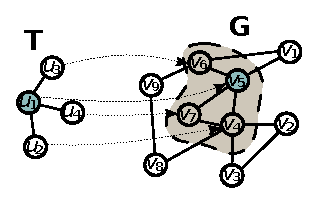
\includegraphics[width=0.35\textwidth]{plots/isomorphism.eps}}
\caption{Here the shaded subgraph is a non-induced embedding of T. The mapping
of the template to the subgraph is denoted with the arrow.}
\label{fig:isomorphism}
\end{figure}

%\subsection{$(\varepsilon,\delta)$-approximation}

\smallskip
\noindent
\textbf{An $(\varepsilon,\delta)$-approximation to $emb(T,G)$.}
We say that a randomized algorithm $\mathcal{A}$ produces an
\emph{$(\varepsilon,\delta)$-approximation} to $emb(T,G)$, if the estimate $Z$
produced by $\mathcal{A}$ satisfies: $\Pr[|Z-emb(T,G)|>\varepsilon \cdot
emb(T,G)]\leq 2\delta$; in other words, $\mathcal{A}$ is required to produce an
estimate that is close to $emb(T, G)$, with high probability.

\smallskip
\noindent
\textbf{Problems studied.}
We consider the following two problems:
\begin{enumerate}
\item
\emph{Subgraph counting}: 
Given a template $T$ and graph $G$, compute an $(\varepsilon,\delta)$-approximation to $emb(T,G)$.
When the labels can be disregarded, we refer to this as the \emph{Unlabeled Subgraph Counting}
problem. Otherwise, it is referred to as the \emph{Labeled Subgraph Counting} problem.
\item
\emph{Graphlet Frequency Distribution (GFD)}~\cite{przulj2007biological}:
a graphlet is another name for a subgraph. We say a node touches a graphlet $T$,
if it is contained in an embedding of $T$ in the graph $G$. The
graphlet degree of a node $v$ is the number of graphlets it touches.
Given a size parameter $k$, the GFD in a graph $G$ is the frequency distribution
of the graphlet degrees of all nodes with respect to all graphlets of size up to $k$. 
The specific problem is to obtain an approximation to the GFD.
In this paper, we will focus on ``treelets'', which only considers all trees of size up to $k$.
\end{enumerate}

\subsection{MapReduce, Hadoop and Harp}
\label{sec:intro-map-reduce}

MapReduce and its extensions have become a dominant computation model
in big data analysis.  It involves two stages for data processing: (a)
divide the input into distinct \emph{map} tasks and distribute to
multiple computing entities, and (b) merging the results of individual
computing entities in the \textit{reduce} tasks to produce the final
output~\cite{dean2008mapreduce}.

The MapReduce model processes data in the form of key-value pairs
$\langle k, v \rangle$. An application first takes pairs of the form
$\langle k_1, v_1 \rangle$ as input to the map function, in which one or
more $\langle k_2, v_2 \rangle$ pairs are produced for each input
pair.  Then the MapReduce re-organizes all $\langle k_2, v_2 \rangle$
pairs and aggregates all items $v_2$ that are associated with the same
key $k_2$, which are then processed by a reduce function.

Hadoop~\cite{white2010hadoop} is an open-sourced implementation of
MapReduce.  By defining application specific map and reduce functions,
the user can employ Hadoop to manage and allocate appropriate
resources to perform the tasks, without knowing the complexity of load
balancing, communication and tasks scheduling. Due to the reliability
and scalability in handling vast amount of computation in parallel,
Hadoop is becoming a \emph{de facto} solution for large parallel
computing tasks.

Hadoop falls short in two aspects though: ({\it i}) the high I/O cost
involved within mapper, shuffling and reducer since the data is always
read and write from the disk in every stage of a Hadoop job and ({\it ii})
global synchronization in mapper and reducer, i.e. reducers can start
only when all mappers have completed their tasks and vice versa,
reduce the efficient usage of the computing resources. To conquer the
problems that Hadoop is facing, we further extends our work to use the
Harp platform~\cite{qiu2014towards}.

Harp introduces full collective communication (broadcast, reduce,
allgather, allreduce, rotation, regroup or push \& pull), adding a
separate communication abstraction. The advantage of using in-memory
collective communication replacing the shuffling phase is that
fine-grained data alignment and data transfer of many synchronization
patterns can be optimized.

Harp categorizes four types of computation models (Locking, Rotation,
Allreduce, Asynchronous) that are based on the synchronization
patterns and the effectiveness of the model parameter update. They
provide the basis for a systematic approach to parallelizing iterative
algorithms. Since the ``Rotation'' model partitions the global model
parameters among distributed workers, it effectively reduces the
memory footprint but requires model synchronization using collective
communication. Figure~\ref{fig:harp} shows the four categories of the
computing model.

\begin{figure}[htbp]
\centerline{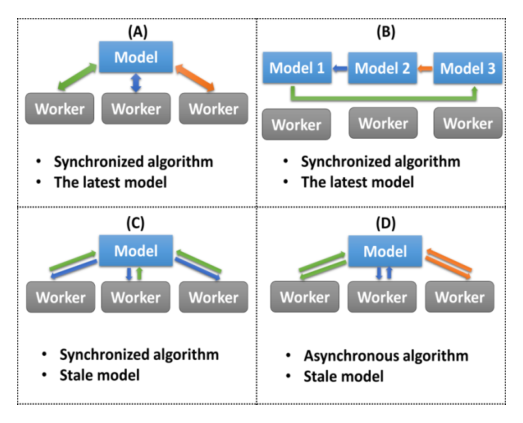
\includegraphics[width=0.35\textwidth]{plots/harp.eps}}

\caption{Harp has 4 computation models: (A) Locking,(B)Rotation, (C) AllReduce, (D) Asynchronous}

\label{fig:harp}
\end{figure}

The Harp framework has been used by 350 students at Indiana University
for their course projects. Now it has been released as open source
project that is available at public github domain
\cite{Web:harp}. Harp provides a collection of iterative machine
learning and data analysis algorithms (e.g. Kmeans, Multi-class
Logistic Regression, Random Forests, Support Vector Machine, Neural
Networks, Latent Dirichlet Allocation, Matrix Factorization,
Multi-Dimensional Scaling) that have been tested and benchmarked on
OpenStack Cloud and HPC platforms including Haswell and Knights
Landing architectures. It has also been used for Subgraph mining,
Force-Directed Graph Drawing, and Image classification applications.



\section{The sequential algorithm: Color Coding}
\label{sec:sequential}


\begin{table}[hptb]
\caption{Notations}
\label{tab:notations}
\centering{
\begin{tabular}{c|c|c|c}
\hline
symbol & description & symbol & description \\
\hline
$G$ & graph & $T, T', T''$ & template and sub-templates \\
$n, m$ & \# nodes, \# edges & $k$ & \# nodes in $T$ \\
$\rho$ & root of $T$ & $S, s_i$ & color set, the $i^{th}$ color \\
$d(v)$ & degree of node $v$ & $N(v)$ & neighbors of node $v$ \\
\hline
\end{tabular}
}
\end{table}



%\subsection{Color Coding for Subgraph Counting}
%\label{subsec:intro-color-coding}

We briefly introduce the color coding algorithm for subgraph
counting~\cite{alon1995color}, which gives a randomized approximation scheme for
counting trees in a graph.  Some of the notation used in the paper is listed in
Table~\ref{tab:notations}.

\noindent
\textbf{High level description.}
There are two main ideas underlying the color coding algorithm of~\cite{alon1995color}.
\begin{enumerate}[leftmargin=4mm, noitemsep, topsep=0pt]
\item
\textbf{Colorful embeddings}:

Color the nodes of the graph with $k$ colors where $k \geq |V_T|$, and only count
``colorful'' embeddings---an embedding $H$ of the template $T$ is colorful if
each node in $H$ has a distinct color.  The advantage of this is that the number
of colorful embeddings can be counted by a simple and natural dynamic program.

\begin{enumerate}
\item
In particular, let $C(v, T(\rho), S)$ be the number of colorful embeddings of $T$ with node
$v \in V_G$ mapped to the root $\rho$, and using the color set $S$, where
$|V_{T}| = |S|$. 
\item
Suppose $(\rho=u_1, u_2)$ is an edge incident on the root node
$\rho$ in $T$. Let tree $T$ be partitioned into trees $T_1$ and $T_2$ when the
edge $(u_1, u_2)$ is removed, with roots $\rho_1=u_1$ and $\rho_2=u_2$ of the
trees $T_1$ and $T_2$, respectively.
\item
Suppose $S_1$ and $S_2$ are disjoint subsets of colors
such that $|S_1|=|V_{T_1}|$, $|S_2| = |V_{T_2}|$. Let $H_1$ and $H_2$ be two
colorful embeddings of $T_1$ and $T_2$ using color sets $S_1$ and $S_2$, respectively,
with $\rho_1$ and $\rho_2$ mapped to neighboring nodes $v_1\in V_G$ and
$v_2\in V_G$, respectively. Then, $H_1$ and $H_2$ must be \emph{non-overlapping},
because they have distinct colors.
\item
Therefore, 
\begin{align*}
C(v_1, T, S) & = \sum_{v_2\in N(v_1)} \sum_{S=S_1\cup S_2} C(v_1, T_1(v_1), S_1) \cdot\\
& \qquad \qquad \qquad \qquad  \qquad C(v_2, T_2(v_2), S_2),
\end{align*}
where the first summation is over all neighbors $v_2$ of $v_1$ and the
second summation is over all partitions $S_1\cup S_2$ of $S$.
\end{enumerate}
\item
\textbf{Random colorings}:
If the coloring is done randomly with $k=|V_T|$ colors, there is a reasonable
probability $\frac{k!}{k^k}$ that an embedding is colorful---this allows us to
get a good approximation to the number of embeddings.
\end{enumerate}

%Figure~\ref{fig:paths} shows an example of the quantities
%$C(v, T_i(\rho_i), S_i)$, and a recurrence relation for computing them, using
%the counts corresponding to smaller trees.  The complete algorithm (described
%below) involves (i) partitioning the template into sub-templates, and (ii) a
%dynamic program to compute the colorful counts.

\begin{algorithm}[ht]
  \caption{The sequential color coding algorithm.}
  \label{alg:sequential}
  \begin{algorithmic}[1]
\STATE \textbf{Input:} Graph $G=(V, E)$ and template $T=(V_T, E_T)$
\STATE \textbf{Output:} Approximation to $emb(T, G)$
\STATE
\STATE For each $v\in V_G$, pick a color $c(v)\in S=\{1,\ldots,k\}$ uniformly at random,
where $k=|V_T|$.

\STATE Partition the tree $T$ into subtrees recursively to form a set $\mathcal{T}$
using algorithm \textsc{Partition}$(T(\rho))$. For each tree $T'\in\mathcal{T}$,
we have a root $\rho'$. Further, if $|V_{T'}|>1$, $T'$ is partitioned into
two trees $T'_1, T'_2$ with roots $\rho'_1=\rho'$ and $\rho'_2$, respectively,
which are referred to as the active and passive children of $T'$.

\STATE For each $v\in V_G$, $T_i\in\mathcal{T}$ with root $\rho_i$, and subset $S_i\subseteq S$,
with $|S_i|=|T_i|$, we compute $C(v, T_i(\rho_i), S_i)$ using the the recurrence
(~\ref{eq:color-coding-dp}) below:

\begin{equation}
\label{eq:color-coding-dp}
\begin{array}{lcl}
\hspace*{-0.2in}c(v, T_i(\rho_i), S_i) = \frac{1}{d}\displaystyle\sum\limits_{u}
\displaystyle\sum c(v, T_i'(\rho_i), S_i') \cdot\\
\hspace*{1.4in}c(u, T_i''(\tau_i), S_i''),
\end{array}
\end{equation}

where $d$ is equal to one plus the number of siblings of
$\tau_i$ which are roots of subtrees isomorphic to $T_i''(\tau_i)$.

\STATE For the $j$th random coloring, let
\begin{equation}
\label{eq:color-coding-sum}
\begin{array}{lcl}
C^{(j)} = \frac{1}{q}\frac{k!}{k^k}\sum_{ v \in V_G} c(v, T(\rho), S),
\end{array}
\end{equation}
where $q$ denotes the number of node $\rho' \in
V_T$ such that $T$ is isomorphic to itself when $\rho$ is mapped to $\rho'$.

\STATE
Repeat the above steps $N=O(\frac{e^k\log(1/\delta)}{\varepsilon^2})$ times,
and partition $N$ estimates $C^{(1)},...,C^{(N)}$ into $t=O(\log(1/\delta))$ sets. Let
$Z_j$ be the average of set $j$. Output the median of $Z_1,...,Z_t$.
  \end{algorithmic}
\end{algorithm}



\begin{algorithm}[ht]
 \caption{\emph{Partition($T(\rho)$)}}
 \label{alg:partition}
\begin{algorithmic}[1]
 \IF{$T \notin \mathcal{T}$}
  \IF{$|V_T| = 1$}
    \STATE $\mathcal{T} \leftarrow T$
  \ELSE
   \STATE Add $T$ to $\mathcal{T}$
   \STATE Pick $\tau \in N(\rho)$, the set of the neighbors of $\rho$,
and partition $T$ into two sub-templates by cutting the edge $(\rho, \tau)$

   \STATE Let $T'$ be the sub-template containing $\rho$ (name as \textit{active child}) and
$T''$ the other (name as \textit{passive child})

   \STATE Partition($T'(\rho)$)
   \STATE Partition($T''(\tau)$)
  \ENDIF
 \ENDIF
\end{algorithmic}
\end{algorithm}


%The sequential color coding algorithm is proposed first in~\cite{alon1995color}
%by Alon \emph{et al.} in 1995. It is a randomized approximation algorithm which
%converges with running time
%$O(m|E|2^me^m\log{(1/\delta)}\frac{1}{\varepsilon^2})$, where $\varepsilon$ and
%$\delta$ are error and confidence parameters, respectively. It consists of the
%following three steps:
%
%\begin{enumerate}
%
%\item Randomly color the nodes in graph $G$ with a color set $S$ which contains $m$
%colors, where $m = |V_T|$, 
%
%\item Using dynamic programming, compute the number of ``colorful''
%embeddings of template $T$, denoted as $c$. A subgraph is colorful if each of
%its node has distinct color.  The dynamic programming is represented by Eq.
%~\ref{eq:color-coding-dp}.
%
%\begin{equation}
%\label{eq:color-coding-dp}
%\begin{array}{lcl}
%
%\hspace*{-0.2in}c(v, T_i(\rho_i), S_i) = \frac{1}{d}\displaystyle\sum\limits_{u}
%\displaystyle\sum c(v, T_i'(\rho_i), S_i') \cdot\\
%\hspace*{1.4in}c(u, T_i''(\tau_i), S_i'')
%
%\end{array}
%\end{equation}
%
%Here, the notation $c(v, T_i(\rho_i), S_i)$ represents the number of the colorful
%subgraphs in $G$ that are isomorphic to $T_i$ (rooted at $\rho$) with $\rho$
%mapped to $v \in G$, and each embedding is colored with $S_i$. The first
%summation is over all $u \in neighbor(v)$ and the second summation is over all $S_i',
%S_i''$ such that $S_i' \cap S_i'' = \emptyset, S_i' \cup S_i'' = S_i$. Here $d$
%is the over-counting factor and is equal to one plus the number of siblings of
%$\tau_i$ which are roots of subtrees isomorphic to $T_i''(\tau_i)$.
%
%\item After dynamic programming, we have $c(v, T(\rho), S)$ for all $v \in
%V_G$. Then we can compute the total number of colorful embeddings with Eq.
%~\ref{eq:color-coding-sum}.
%
%\begin{equation}
%\label{eq:color-coding-sum}
%\begin{array}{lcl}
%C = \frac{1}{q}\sum_{\forall v \in V_G} c(v, T(\rho), S)
%\end{array}
%\end{equation}
%
%Here $q$ is another over counting factor, i.e., the number of node $\rho' \in
%V_T$ such that $T$ is isomorphic to itself when $\rho$ is mapped to $\rho'$.
%
%
%\item Suppose the number of all embeddings of $T$ is $Y$, then it is easy to
%obtain $C = Y \cdot \frac{m!}{m^m}$, therefore, we can compute $Y = C \cdot
%\frac{m^m}{m!}$. 
%
%\end{enumerate}

Algorithm~\ref{alg:sequential} describes the sequential color coding algorithm.
Figure~\ref{fig:example-dp} gives an example of computing Eq. 1.

\begin{figure}[htbp]
\centerline{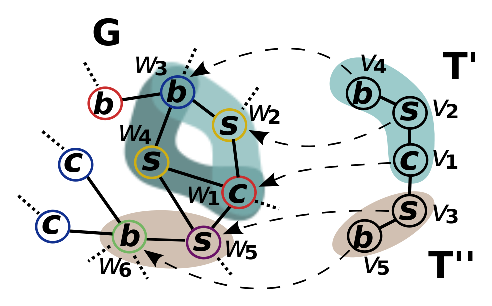
\includegraphics[width=0.24\textwidth]{plots/paths.eps}}

\caption{The example shows one step of the dynamic programming in color coding.
$T$ in Figure~\ref{fig:isomorphism} is split into $T'$ and $T''$. To count
$C(w_1, T(v_1), S)$, or the number of embeddings of $T(v_1)$ rooted at $w_1$,
using color set $S=\{\underline{r}ed, \underline{y}ellow, \underline{b}lue,
\underline{p}urple, \underline{g}reen\}$, we first obtain $C(w_1, T'(v_1), \{r,
y, b\})=2$ and $C(w_5, T''(v_3), \{p, g\})=1$.  Then, $C(w_1, T(v_1), S) =
C(w_1, T'(v_1), \{r, y, b\}) C(w_5, T''(v_3), \{p, g\})=2$.  The
embeddings of $T$ are subgraphs with nodes $\{w_3, w_4, w_1, w_5, w_6\}$ and
$\{w_3, w_2, w_1, w_5, w_6\}$. Here $s, c, b$ represents the label of the nodes.
Details of labeled subgraph counting can be found at~\cite{zhao2012sahad}.}

\label{fig:example-dp}
\end{figure}

 
\section{Parallel algorithms}
\label{sec:parallel}

In this section, we present a parallelization of the color coding approach using
MapReduce framework, we will first describe \sahad{}
\cite{zhao2012sahad}, followed by  \ensahad{} and  \harpsahad{} respectively.

\subsection{\sahad{}}
\label{sec:sahad-implementation}

\sahad{} takes a sequence of templates $\mathcal{T}=\{T_0,...,T\}$ as
input. Here $\mathcal{T}$ represents a set of templates generated by
partitioning $T$ using Algorithm~\ref{alg:partition}. Then it performs MapReduce
variation of Algorithm~\ref{alg:sequential} to compute the number of embeddings
of $T$. 

As shown in Equation~\ref{eq:color-coding-dp}, the counts of all colorful embeddings
isomorphic to $T$ rooted from a single node $v$ is computed by aggregating the
same measurement of $T'$ and $T''$, i.e., the two sub-templates, with $T'$
rooted from $v$ and $T''$ rooted from $\forall u \in N(v)$. We can parallelize
color-coding algorithm by distributing the computation among multiple machines,
and sending data related with $v$ and $N(v)$ to a computation unit for the
aggregation. In our MapReduce algorithm, we manage this by assigning $v$ as the
key for both the counts of $T'$ rooted at $v$ and the counts of $T''$ rooted
at $v$'s neighbors, such that all data required for computing counts for
$T$ rooted at $v$ has the same key and will be handled by a single reduce
function.

%We hereby define the notation $X_{T, v}$ since we will be using it in the
%algorithms presented in this paper. 
Let $X_{T, v}$ be a sequence of color-count
pairs $(S_0=\{s_1^0, s_2^0, ..., s_k^0\}, c_0), (S_1=\{s_1^1, s_2^1, ...,
s_k^1\}, c_1),...$, where $S_i$ represent a color set containing $k$ colors, and
$c_i$ is the counts of the subgraphs isomorphic to $T$ and rooted at $v$ that
are colored by $S_i$. Here $k = |V(T)|$, and each subgraph is a colorful match.

There are 3 types of Hadoop jobs in \sahad{}, which are 1) colorer
(Algorithm~\ref{alg:colorer-mapper}) that performs line 4 of Algorithm
~\ref{alg:sequential}; 2) counter (Algorithm~\ref{alg:counter-mapper},
~\ref{alg:counter-reducer}) which performs line 6 of Algorithm
~\ref{alg:sequential} and 3) finalizer (Algorithm~\ref{alg:sum-mapper},
~\ref{alg:sum-reducer}) that performs line 7 of Algorithm~\ref{alg:sequential}. 

The first step is to random color network $G$ with $k$ colors. The map function 
is described in Algorithm~\ref{alg:colorer-mapper}:

\begin{algorithm}[ht]
  \caption{\emph{mapper($v, N(v)$)}}
  \label{alg:colorer-mapper}
  \begin{algorithmic}[1]
    \STATE Pick $s_i \in \{s_1,\ldots,s_k\}$ uniformly at random\\
	\STATE color $v$ with $s_i$
	\STATE Let $T_0$ be the single node template
	\STATE Let $c(v, T_0, \{s_i\})=1$ since $v$ is the only colorful matching\\
    \STATE $X_{T_0, v} \leftarrow \{(\{s_i\}, 1)\}$ \\
    \STATE Collect($\underline{key \leftarrow v}, \underline{value \leftarrow X_{T_0, v}, N(v)}$)
  \end{algorithmic}
\end{algorithm}

Here ``Collect'' is a standard MapReduce operation that will emit the key-value
pairs to global space for further process such as shuffling, sorting or I/O.
$N(v)$ represents the neighbors of $v$. Note that template $T_0$ is a single
node, therefore $X_{T_0, v}$ contains only a single color-count pair $({s_v}, 1)$

According to Equation~\ref{eq:color-coding-dp}, to compute $X_{T_i, v}$, we need $X_{T'_i, v}$ for
sub-template $T'_i$ and $X_{T''_i, u}$ for all $u \in N(v)$ for sub-template
$T''_i$. We use a mapper and a reducer function to implement this as shown in
Algorithm~\ref{alg:counter-mapper} and \ref{alg:counter-reducer}, respectively.

\begin{algorithm}[ht]
  \caption{\emph{mapper($v, X_{t, v}, N(v)$)}}
  \label{alg:counter-mapper}
  \begin{algorithmic}[1]
    \IF{$t$ is $T'_i$}
      \STATE Collect($\underline{key \leftarrow v}, \underline{value \leftarrow X_{t, v}, flag'}$)
    \ELSE
      \FOR{$u \in N(v)$}
        \STATE Collect($\underline{key \leftarrow u}, \underline{value \leftarrow X_{t, v}, flag''}$)
      \ENDFOR
    \ENDIF
  \end{algorithmic}
\end{algorithm}

Note that in Algorithm~\ref{alg:counter-mapper}, the second \textit{Collect} emits
$X_{T''_i, v}$ to all its neighbors. Therefore, as shown in Algorithm
~\ref{alg:counter-reducer}, $X_{T'_i, v}$ and $X_{T''_i, u}$ from all $u \in
N(v)$ are handled by the same reducer, which is sufficient for computing Eq.
~\ref{eq:color-coding-dp}. Also note that for a given node
$v$, the number of entries with $flag'$ is 1, and the number of entries with
$flag''$ equals $|N(v)|$.


\begin{algorithm}[ht]
  \caption{\emph{reducer($v, {(X, flag), (X, flag), ...}$)}}
  \label{alg:counter-reducer}
  \begin{algorithmic}[1]
    \STATE pick $X_1$ where $flag = flag'$
      \FOR {all colorset $S'_i$ from $X_1$}
 \FOR {each $X$ other than $X_1$} 
   \FOR {all colorset $S''_i$ from $X$}
     \IF {$S'_i \cap S''_i = \emptyset$}
              \STATE $c(v, T_i, S'_i \cup S''_i) += 1$
            \ENDIF
          \ENDFOR
        \ENDFOR
      \ENDFOR 
    \STATE Collect($\underline{key \leftarrow v}, \underline{value \leftarrow X_{T_i, v}, N(v)}$)
  \end{algorithmic}
\end{algorithm}

The last step is to compute the total count described in Eq.
~\ref{eq:color-coding-sum}, and is shown in Algorithm \ref{alg:sum-mapper} and
~\ref{alg:sum-reducer}.

\begin{algorithm}[ht]
  \caption{\emph{mapper($v, X_{T, v}, N(v)$)}}
  \label{alg:sum-mapper}
  \begin{algorithmic}[1]
      \STATE Collect($\underline{key \leftarrow ``sum''}, \underline{value \leftarrow X_{T, v}}$)
  \end{algorithmic}
\end{algorithm}

\begin{algorithm}[ht]
  \caption{\emph{reducer($``sum'', {X_{T, v_1}, {X_{T, v_2},...}}$)}}
  \label{alg:sum-reducer}
  \begin{algorithmic}[1]
    \STATE $Y = \frac{m^m}{m!} \cdot \frac{1}{q}\sum_{\forall v \in V_G}X$
    \STATE Collect($\underline{key \leftarrow ``sum''}, \underline{value \leftarrow X_{T, v}}$)
  \end{algorithmic}
\end{algorithm}

Note that in Algorithm~\ref{alg:sum-mapper}, $X_{T,v}$ only contains one
element, which is the count corresponding to the entire color set. Then in the
reducer shown in Algorithm~\ref{alg:sum-reducer}, all the counts are added
together and properly factorized, to obtain the final count. For a
comprehensive description of the MapReduce version of color coding, please
refer to~\cite{zhao2012sahad}.

\subsection{\ensahad}
\label{sec:ensahad}

For general MapReduce problem, the set of keys that is processed in Mapper and
Reducer varies among different jobs. Therefore, MapReduce uses external
shuffling and sorting in-between Mappers and Reducers to deploy the keys to
computing nodes. 

In our algorithm, however, the dynamic programming aggregates counts based on
the root node of the subtree, and therefore the key is the node index $v$.  In
\ensahad{}, we use this pre-knowledge to predefine a reducer that is
corresponding to a set of nodes. We also assign the predefined reducers to
computing nodes prior to the beginning of the dynamic programming. Therefore, a
data entry with key $v$ will be directly sent to the corresponding computing
node and processed by designated Reducer. Using this mechanism, we can reduce
the cost of shuffling and sorting in intermediate stage of Hadoop jobs.

\iffalse
In addition, the network communication cost among computing nodes is also a
bottleneck in most of the parallellization frameworks. With the predefined
reducers, the communication cost is $O(E_{out})$. Here $E_{out}$ represents the
number of edges among partitions. To study the performance variations regarding
$E_{out}$, we explore different partitioning schemes for distributing graph data
to computing nodes.  Some partitioning schemes may introduce lower number of
inter-partition edges $E_{out}$, but higher number of intra-partition edges.
Here we investigate two partitioning schemes: the random partitioning and
min-cut partitioning.

We use~\cite{Web:metis} to perform minimum cut partitioning with the following
two constraints: a) divide the network into partitions with roughly the same
size, b) minimize the number of inter-partition edges. The purpose is to
maintain load balancing among computing nodes, and reduce the communication cost
$O(E_{out})$ by minimizing the number of inter-partition edges.

\fi


\subsection{\harpsahad{}}
\label{sec:harp-implementation}

\begin{figure}[htbp]
\centerline{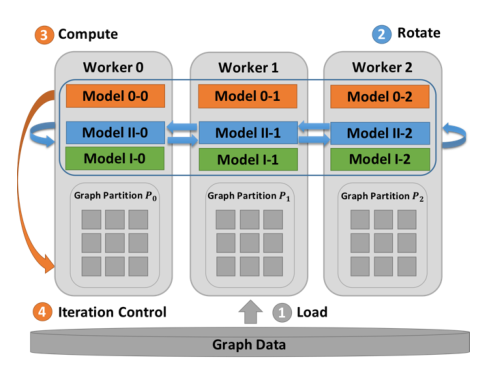
\includegraphics[width=0.36\textwidth]{plots/harp-imp.eps}}
\caption{Here shows one iteration of the Harp implementation. $P_0$ through
$P_2$ are parts of a partition of graph $G$}
\label{fig:harp-imp}
\end{figure}


Figure~\ref{fig:harp-imp} illustrates \harpsahad{} for one iteration
that counts the embeddings of the template $T$ based on the embeddings of
sub-template $T'$ and $T''$.  Graph data is partitioned and stored separately on
each worker node in the form of adjacency list. Partitioned graph data is loaded
and cached in memory. The model represents a data structure including a
color-count pairs for each vertex in graph. Since it follows the dynamic
programming scheme, computation runs with static partitioned graph and multiple
template models. Model updates are achieved with Model I (embeddings of
sub-template $T'$) and model II (embeddings of sub-template $T''$) generating
embeddings of template $T$ on model 0. Note that model I and model II are
partitioned and stored separately on the cluster. The model distribution
approach with rotation can effectively reduce memory usage per node, thereby
addressing the issue when graph template models become too large to fit into
memory.


Note that only model II rotates among the worker nodes. As such, it takes three
rounds to complete updating model 0 in Figure~\ref{fig:harp-imp}. In the first round, 
it joins model I-0 and model II-0 to generate new values for model 0-0. Then all
parts of model II
rotate so that model II-2 is accessible on worker 0. In the second round, it
joins model I-0 and model II-2 and updates model 0-0. Again, it rotates so that
model II-1 is now accessible to worker 0. It then joins model I-0 with model II-1
and updates model 0-0. After this rotation, worker 0 is given access to all
parts of model II and complete updating model 0 in one iteration. Worker 1
and worker 2 run in the same way in parallel. At each iteration, the embeddings 
of sub-template $T'$ and $T''$ are used for updating the embeddings of the parent 
template $T$. Harp model rotation achieves scaling for fine-grained graph
model synchronization with in-memory collective communication.


\input{extensions}
\input{experiments}
\input{conclusions}



% if have a single appendix:
%\appendix[Proof of the Zonklar Equations]
% or
%\appendix  % for no appendix heading
% do not use \section anymore after \appendix, only \section*
% is possibly needed

% use appendices with more than one appendix
% then use \section to start each appendix
% you must declare a \section before using any
% \subsection or using \label (\appendices by itself
% starts a section numbered zero.)
%

\iffalse

\appendices
\section{Proof of the First Zonklar Equation}
Appendix one text goes here.

% you can choose not to have a title for an appendix
% if you want by leaving the argument blank
\section{}
Appendix two text goes here.


% use section* for acknowledgment
\ifCLASSOPTIONcompsoc
  % The Computer Society usually uses the plural form
  \section*{Acknowledgments}
\else
  % regular IEEE prefers the singular form
  \section*{Acknowledgment}
\fi


The authors would like to thank...


% Can use something like this to put references on a page
% by themselves when using endfloat and the captionsoff option.
\ifCLASSOPTIONcaptionsoff
  \newpage
\fi

\fi


% trigger a \newpage just before the given reference
% number - used to balance the columns on the last page
% adjust value as needed - may need to be readjusted if
% the document is modified later
%\IEEEtriggeratref{8}
% The "triggered" command can be changed if desired:
%\IEEEtriggercmd{\enlargethispage{-5in}}

% references section

% can use a bibliography generated by BibTeX as a .bbl file
% BibTeX documentation can be easily obtained at:
% http://mirror.ctan.org/biblio/bibtex/contrib/doc/
% The IEEEtran BibTeX style support page is at:
% http://www.michaelshell.org/tex/ieeetran/bibtex/
%\bibliographystyle{IEEEtran}
% argument is your BibTeX string definitions and bibliography database(s)
%\bibliography{IEEEabrv,../bib/paper}
%
% <OR> manually copy in the resultant .bbl file
% set second argument of \begin to the number of references
% (used to reserve space for the reference number labels box)

\bibliographystyle{abbrv}
\bibliography{zz}

% biography section
% 
% If you have an EPS/PDF photo (graphicx package needed) extra braces are
% needed around the contents of the optional argument to biography to prevent
% the LaTeX parser from getting confused when it sees the complicated
% \includegraphics command within an optional argument. (You could create
% your own custom macro containing the \includegraphics command to make things
% simpler here.)
%\begin{IEEEbiography}[{\includegraphics[width=0.8in,height=1in,clip,keepaspectratio]{mshell}}]{Michael Shell}
% or if you just want to reserve a space for a photo:

\begin{IEEEbiography}[{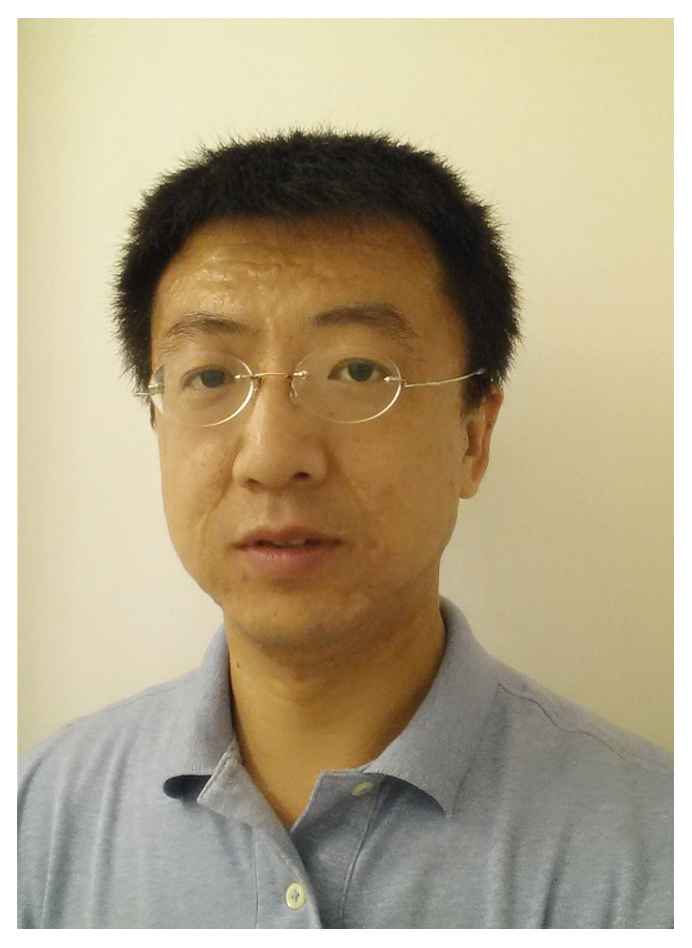
\includegraphics[width=0.8in,height=1in,clip,keepaspectratio]{authors-pic/zhaozhao.eps}}]{Zhao Zhao}
 is pursueing his Ph.D degree in part-time in the Department of
Computer Science, Virginia Tech. He also works as a Software Engineer in
Verisign Labs, Verisign Inc in full time. His research interests lie in the area
of parallel graph algorithms for very large networks. 
\end{IEEEbiography}

\begin{IEEEbiography}[{
\includegraphics[width=0.8in,height=1in,clip,keepaspectratio]{authors-pic/limeng.eps}}]{Meng Li}
 is a Computer Science Ph.D. student in the School of informatics and
Computing at Indiana University. His advisor is Prof. Judy Qiu. His research
interest is distributed systems and parallel computing.
\end{IEEEbiography}

\begin{IEEEbiography}[{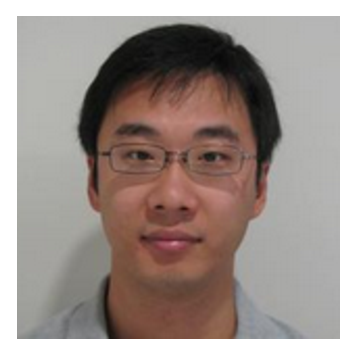
\includegraphics[width=0.8in,height=1in,clip,keepaspectratio]{authors-pic/guanying.eps}}]{Guanying Wang}
 earned his PhD from Virginia Tech in 2012. He is now a software
engineer at Google.
\end{IEEEbiography}

\begin{IEEEbiography}[{
\includegraphics[width=0.8in,height=1in,clip,keepaspectratio]{authors-pic/ali.eps}}]{Ali Butt}
 received his Ph.D. degree in Electrical and Computer Engineering from Purdue
 University in 2006. He is a recipient of an NSF CAREER Award, IBM Faculty
 Awards, a VT College of Engineering (COE) Dean's award for "Outstanding New
 Assistant Professor", and NetApp Faculty Fellowships. Ali's research interests
 are in distributed computing systems and I/O systems.  \end{IEEEbiography}

\begin{IEEEbiography}[{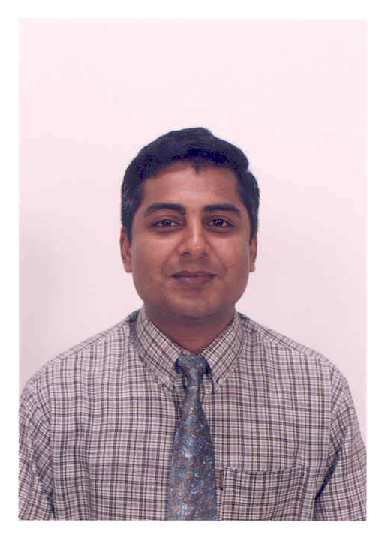
\includegraphics[width=0.8in,height=1in,clip,keepaspectratio]{authors-pic/maleq.eps}}]{Maleq Khan}
 is an Assistant Professor in the Department of Electrical Engineering
and Computer Science at Texas A\&M University - Kingsville. Prior to Joining
this department in August 2016, he worked in Biocomplexity Institute of Virginia
Tech from 2007 to 2016.
\end{IEEEbiography}

\begin{IEEEbiography}[{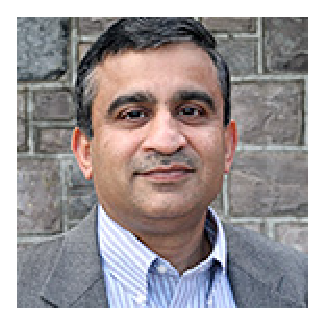
\includegraphics[width=0.8in,height=1in,clip,keepaspectratio]{authors-pic/madhav.eps}}]{Madhav Marathe}
 is a professor of Computer Science and director of the Network
Dynamics and Simulation Science Laboratory. He obtained his Bachelor of
Technology degree in 1989 in Computer Science and Engineering from the Indian
Institute of Technology, Madras, and his Ph.D. in 1994 in Computer Science from
the University at Albany under the supervision of Professors Harry B. Hunt III
and Richard E. Stearns. He also holds adjunct appointments at Chalmers
University, and the Indian Institute of Public Health.
\end{IEEEbiography}

\begin{IEEEbiography}[{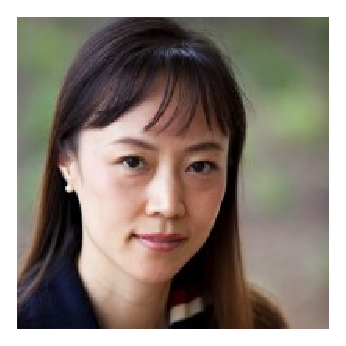
\includegraphics[width=0.8in,height=1in,clip,keepaspectratio]{authors-pic/judy.eps}}]{Judy Qiu}
 is an associate professor of Intelligent Systems Engineering in the
School of Informatics and Computing at Indiana University. Her research
interests are parallel and distributed systems, cloud computing, and
high-performance computing. Her research has been funded by NSF, NIH, Intel,
Microsoft, Google, and Indiana University. Judy Qiu leads the Intel Parallel
Computing Center (IPCC) site at IU. She is the recipient of a NSF CAREER Award
in 2012, Indiana University Trustees Award for Teaching Excellence in 2013-2014,
and Indiana University Outstanding Junior Faculty Award 2015
\end{IEEEbiography}

\begin{IEEEbiography}[{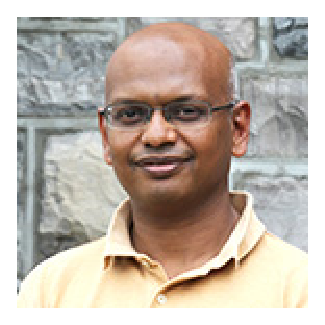
\includegraphics[width=0.8in,height=1in,clip,keepaspectratio]{authors-pic/anil.eps}}]{Anil Vullikanti}
 is an Associate Professor in the Dept. of Computer
Science and Biocomplexity Institute of Virginia Tech. He received his
undergraduate degree from the Indian Institute of Technology, Kanpur, and his
Ph.D. from the Indian Institute of Science, Bangalore. He was a post-doctoral
researcher at the Max-Planck Institute for Informatics, and a Technical Staff
Member at the Los Alamos National Laboratory.
\end{IEEEbiography}

% if you will not have a photo at all:
%\begin{IEEEbiographynophoto}{John Doe}
%Biography text here.
%\end{IEEEbiographynophoto}

% insert where needed to balance the two columns on the last page with
% biographies
%\newpage

% You can push biographies down or up by placing
% a \vfill before or after them. The appropriate
% use of \vfill depends on what kind of text is
% on the last page and whether or not the columns
% are being equalized.

%\vfill

% Can be used to pull up biographies so that the bottom of the last one
% is flush with the other column.
%\enlargethispage{-5in}



% that's all folks
\end{document}


